%%%%%%%%%%%%%%%%%%%% author.tex %%%%%%%%%%%%%%%%%%%%%%%%%%%%%%%%%%%
%
% sample root file for your "contribution" to a proceedings volume
%
% Use this file as a template for your own input.
%
%%%%%%%%%%%%%%%% Springer %%%%%%%%%%%%%%%%%%%%%%%%%%%%%%%%%%


\documentclass{svproc}
%
% RECOMMENDED %%%%%%%%%%%%%%%%%%%%%%%%%%%%%%%%%%%%%%%%%%%%%%%%%%%
%

% to typeset URLs, URIs, and DOIs
\usepackage{url}
\usepackage{color}
\usepackage{makeidx}         % allows index generation
\usepackage{graphicx}        % standard LaTeX graphics tool
\usepackage[misc]{ifsym}                            % when including figure files
\usepackage{multicol}        % used for the two-column index
\usepackage[bottom]{footmisc}% places footnotes at page bottom
\usepackage{tabularx}
\usepackage{multirow}
\usepackage{natbib}
\usepackage{algorithm}
\usepackage{algorithmic}
\usepackage[center]{caption}
\usepackage{longtable}
\usepackage{rotating}
 \usepackage{amsmath}
\usepackage{subfigure}
\def\UrlFont{\rmfamily}

\begin{document}
\mainmatter              % start of a contribution
%
\title{Peregrine Preying Pattern based Differential Evolution}
%
\titlerunning{P3DE}  % abbreviated title (for running head)
%                                     also used for the TOC unless
%                                     \toctitle is used
%
\author{Sanjay Jain\inst{1} \and Vivek Kumar Sharma\inst{1} \and Sandeep Kumar\inst{3}}
%
\authorrunning{Sanjay Jain et al.} % abbreviated author list (for running head)
%
%%%% list of authors for the TOC (use if author list has to be modified)
\tocauthor{Sanjay Jain, Vivek Kumar Sharma, and Sandeep Kumar}
%
\institute{Amity University Rajasthan, Jaipur- 302039 India,\\
\email{jainsanjay17@yahoo.co.in}\\
\and
CHRIST (Deemed to be University), Bangalore-560029, India\\
\email{sandpoonia@gmail.com}
}

\maketitle              % typeset the title of the contribution

\begin{abstract}
The differential evaluation (DE) algorithm is an evolutionary algorithm. It is a popular metaheuristics that efficiently solved various complex optimization problems. This paper proposed modification in DE, motivated by the flying pattern of peregrine falcon while preying and named as peregrine preying pattern based DE algorithm (P3DE). In P3DE, the flying pattern of peregrine improves the exploration potential, while preserving the novel exploitation potential of the DE. The competence, precision, robustness and trustworthiness of the projected P3DE algorithm is analyzed while simulating it over 12 composite benchmark functions of diverse characteristics. The results of P3DE compared with DE and Artificial Bee Colony algorithm to prove its competitiveness for selected problems.
% We would like to encourage you to list your keywords within
% the abstract section using the \keywords{...} command.
\keywords{Evolutionary Algorithm, Logarithmic Spiral, Meta\-heuristics, Nature Inspired Algorithm, Optimization}
\end{abstract}
%
\section{Introduction}\label{sec:intro}
Storn and Price \cite{price1996differential} developed a simple and fast algorithm in year 1995 namely Differential Evolution. The fundamental concept in DE is to make use of the vector differences for perturbing vector solutions. DE is a stochastic meta-heuristic. DE fits into the class of Evolutionary Algorithms (EAs). A number of characteristics like trial vector development procedure (discussed in section \ref{sec:de}) make use of the information about direction and distance from present population to engender a fresh trial vector is significantly contrasting with other existing evolutionary strategies. In case of DE the mutation is applied first and then  crossover applied while in all other EAs, most of the time a trial vector generated using crossover in first step and then one offspring produced using the mutation operation.

DE is very popular among researchers specially working in the field of optimization as it has a number of advantages over other population-based algorithms. But similar to other stochastic algorithms DE also has some drawback and researchers are frequently working to enhance the efficiency and reliability of this evolutionary algorithm. A few recent and most popular variants of DE are discussed  in \cite{chakraborty2008advances} with appropriate applications. DE performs better than the many other 	competitive algorithms like Genetic Algorithm (GA) \cite{holland1975adaptation, kumar2018genetic} and the Particle Swarm Optimization (PSO) \cite{kennedy1995particle} for considered numerical benchmarks \cite{vesterstrom2004comparative} and many more new algorithms \cite{rajpurohit2017glossary}. DE has proved its superiority over other algorithm in various applications of science, management, engineering and technology like chemical engineering \cite{liu2008inverse}, mechanical engineering design \cite{rogalsky2000differential},  machine intelligence, pattern recognition \cite{omran2005differential}, robot path planning \cite{sharma2019black} and signal processing \cite{das2006two}. Now a days DE algorithm is one of the most accepted strategies in area of engineering optimization, machine intelligence and cybernetics.

The evolution of population in DE is driven by variation and selection.  The deviation process is absolutely accountable for the exploration of different areas of the probable search region and exploitation of the finest solution is done by the process of selection. A number of new study shows that sometimes DE is not able to achieve global optimum \cite{lampinen2000stagnation}. In this paper, to set up an appropriate trade-off between diversification and convergence of the population in DE, a natural phenomenon of specific flying pattern exhibited by peregrine falcon while preying is implemented with DE and named as peregrine preying pattern based DE algorithm (P3DE).

\section{Overview of DE Algorithm}\label{sec:de}
The general notation for DE is: $DE/x/y/z$, here DE stands for Differential Evolution, $x$ represents the strategy for selection of target vector, number of differential vector used perturbation of $x$ denoted by $y$, and $z$ represent the crossover technique employed. Based of selection of $x$, $y$ and $z$ \cite{price1996differential} various variant of DE are available. The most popular DE scheme $DE/rand/1/bin$ and also used in this paper. It select the target vector randomly and use binomial crossover with one differential vector.  The DE recognised among researchers as it is very simple, robust, easy in implementation and has wide class of applicability to real world problems \cite{sharma2019review}.

\subsection{Mutation}

The mutation operator generate a trial solution by doing some random changes in trial solution. The working of mutation operator to engender a trial solution $u_i$ from the parent solution $x_i$ is defined as follow:
\begin{itemize}
\item Select a target vector $x_{i_1}(g)$ in such a way that $i$ and $i_1$ are not same.
\item Identify two random solutions, $x_{i_2}$ and $x_{i_3}$ in such a way that $i$, $i_1$, $ i_2$ and $i_3$ are different.
\item The trial vector computed by mutating target vector using equation \ref{eq:modpos}

\begin{equation}\label{eq:modpos}
u_i(g)= x_{i_1}(g)+ F\times (x_{i_2}(g)-x_{i_3}(g))
%u_i(G)= x_{i_1}(G)+underbrace{F\times \overbrace{(x_{i_2}(G)-x_{i_3}(G))}^{\hbox{Variation Component}}}_{\hbox{Step size}}
\end{equation}

where mutation scale factor $F \in [0, 1]$ control the escalation of the differential variation \cite{engelbrecht2007computational}.
\end{itemize}

\subsection{Crossover}
DE apply uniform crossover to engender offspring $x'_i(g)$ using parent vector, $x_i(g)$ and the trial vector, $u_i(g)$ as follows:
\begin{equation}
    x'_{ij}(g)=\begin{cases}
                    u_{ij}(g), &  \mbox{if } j\in J\\
                    x_{ij}(g), & \mbox{otherwise}.
                \end{cases}
\end{equation}
where a set of crossover points denoted by $J$, $j^{th}$ element of $x_i(g)$ vector denoted by $x_{ij}(g)$. It is supposed that if $j\in J $ , the trial parameter is selected from the mutant $u_{ij}(g)$.

\subsection{Selection}

The selection operator decides between trial vector and target vector. It decides the individual to compute the trial vector for the mutation and precisely choose the best for the next generation, between the trial vector and their predecessors based on their fitness value. If fitness of trial vector is lower than target vector then it takes over from the target vector for next generation. Contrarily, the target vector $x_{i}(g)$ remains there for next generation i.e. best fitted individual selected for next generation.
\begin{equation*}
    x_{i}(g+1)=\begin{cases}
                    x'_{i}(g), &  \mbox{if } f( x'_{i}(g))>f(x_{i}(g)).\\
                    x_{i}(g), & \mbox{else}.
                \end{cases}
\end{equation*}

In order to mend the results of basic DE, researchers have proposed a number of variants of DE. It has been observed by Storn and Price in \cite{price1996differential} that the best suitable range for value of $F$ is [0.5, 1] and $[5D, 10D]$ is the most appropriate range of the value of $NP$, where, considered problem is of $D$ dimension.

Most of the researchers focused on identification of best suitable value for control parameters ($F$ and $CR$) but very few researchers tried to identify the best suitable size of the population ($NP$) for performance enhancement. New variants of DE proposed by Teo \cite{teo2006exploring} and Sharma et al. \cite{sharma2012dynamic} based on the concept of self adaption in populations and dynamic scaling. They suggested self adaption in order to avoid manual parameter setting. Some new strategies also incorporated in DE like: opposition based strategy \cite{kumar2014opposition}, fitness based strategy \cite{sharma2012fitness}, convex mutation \cite{sharma2016asynchronous}, memetic search \cite{kumar2014memetic} and position update \cite{jain2017improved}. Some modifications in population selection suggested by researchers \cite{sharma2015modified}.

\section{Peregrine Preying Pattern based DE Algorithm} \label{P3DE}
The peregrine falcon is one of the most intelligent raptor from the falconidae family of birds that hunts and feeds on rodents and other animals. Peregrine falcons has two important skills, first is flight with speed over 200 mph and visual sharpness that are very helpful while attacking their prey. Peregrine falcons are found worldwide. The peregrine follows a particular path while chasing prey and it is similar to logarithmic spiral. The studies reveal that peregrine falcons follow a logarithmic spiral path to attack their prey \cite{lorimer2006curved, ls2018}. The peregrine flees along a logarithmic spiral route to avoid the conflict between vision and aerodynamics \cite{tucker2000curved}.

This paper presents an improved mutation strategy inspired by the path followed by peregrine falcon during attack on prey i.e. logarithmic spiral. It is a self-similar spiral curve which formed by peregrine falcon while preying \cite{ls2018}. As the solution search process of DE algorithm is highly depends on a combination of randomly selected vectors and a difference vector (refer equation \ref{eq:modpos}). Hence, there are more chances to omit the true solution in case of high value of scaling factor $F$ and the difference vector. Therefore, here a new approach to decide scaling factor proposed, which helps the current best solution in the swarm to exploit the potential solutions in its vicinity.

The equation of logarithmic spiral is shown in equation \ref{eq:lsmain}. It is the locus of points going apart from a centre point with a invariable speed besides a line which rotates with fixed angular velocity proportional to the positions with time of a point. Unvaryingly, in polar coordinates $(r, \theta)$ as illustrated by the equation \ref{eq:lsmain} \cite{ls2018}.
\begin{equation}\label{eq:lsmain}
    r = a\times e^{b\theta}\,
\end{equation}

Here, $a$ and $b$ are real numbers while $e$ denotes the base of natural logarithms. The parameter $a$ control the turning of the spiral and the distance between consecutive turnings managed by $b$ as shown in Figure \ref{fig:asfig}.
\begin{figure}[h!]
\begin{center}
    %\centering
     
\includegraphics[width=0.4\textwidth]{ls.eps}
    \caption{Logarithmic spiral \cite{ls2018}}
     \label{fig:asfig}
\end{center}
\end{figure}

In P3DE, the best solution in the current pool of solution is permitted to modernize their position adaptively. The new mutation approach is developed by taking inspiration from the logarithmic spiral as shown in equation \ref{eq:asu}.
%u_i(G)= x_{i_1}(G)+ F\times (x_{i_2}(G)-x_{i_3}(G))
\begin{eqnarray}
% \nonumber to remove numbering (before each equation)
  u_i(g)&=& x_{i_1}(g)+ \mbox{$F_{P3DE}$}\times (x_{i_2}(g)-x_{i_3}(g))\label{eq:asu}\\
  %x_{new} &=& x_{best}+ \mbox{ step}\label{eq:asu} \\
  \mbox{where, $F_{P3DE}$ } &=& 2\times sign\times U(0,1)\times (1-\frac{Iter}{TI}) \times e^{\frac{sin(Iter)}{Iter}} \label{eq:asu1}
\end{eqnarray}
Here, $Iter$ is the counter for search iteration, $TI$ represents total number of iterations, $sign$ is the addition or subtraction sign which depends on the fitness of the new solution. The scale factor is calculated using equation  \ref{eq:asu1} which is developed by modification of logarithmic spiral equation. In this equation $a=2\times sign\times U(0,1)\times (1-\frac{Iter}{TI})$ and $\theta=sin(Iter)$. The step size is used to provide distance to the best individual during the search process.

\section{Experimental results and discussion}\label{sec:exp}
The performance of newly developed variant (P3DE) evaluated over thirteen unbiased standard problems and analysed here in terms of precision, efficacy and trustworthiness. A set of $12$ mathematical optimization problems with diverse degree of complexity are selected to confirm the proficiency of the planned P3DE algorithm. All the selected functions are continuous in nature. These problems are minimization problems and solutions of the most of the functions does not exists on the origin, diagonal and axis.

\subsection{Experimental setting}\label{sec:setting}
In order to check the performance of P3DE, initial population (N) was taken $50$ and number of iterations ($itr$) taken as $4000$. The newly developed P3DE algorithm is compared with basic DE \cite{storn1995differential} and ABC \cite{karaboga2005idea} for the purpose of assessment to evaluate the efficiency, robustness and reliability. Simulation results of the newly developed P3DE algorithm and the considered algorithms are presented in terms of success rate (SR), average number of function evaluations (AFE) and mean error (ME) as mentioned in Tables \ref{lsabctable:sr}, \ref{lsabctable:afe} and \ref{lsabctable:me} respectively. Standard deviation (SD) also measured for analysis. The considered algorithms are examined with the following experimental setting:

\subsection{Results Analysis of Experiments}\label{sec:comp}
To evaluate the efficiency, an AFE based comparison is depicted out in Table \ref{lsabctable:afe}. It can be easily observed from this table that the AFE of P3DE is less for most of the functions i.e. the newly developed P3DE is converge to optima faster than the other considered algorithms. Further, the Table \ref{lsabctable:sr} shows the results of successful runs over 100 simulations. A simulation is considered successful, if the algorithm achieves optima at the level of acceptable error. The Table \ref{lsabctable:sr} elucidate that the newly developed P3DE is more reliable for most of the benchmark functions in terms of success rate as compared to the considered algorithms. The robustness and accuracy of the newly developed P3DE algorithm is measured by the ME as depicted in Table \ref{lsabctable:me}. This table exhibits competitiveness of the purposed algorithm in terms of accuracy for the considered Test Problems (TP).


\begin{table}
\centering
\minipage{0.45\textwidth}
\caption{Comparison based on AFE.}
\label{lsabctable:afe}
\resizebox{\linewidth}{!}{%
\begin{tabular}{|p{3.1cm}|p{1.4cm}|p{1.3cm}|p{1.3cm}|}
\hline
 {TP} & {ABC} &  {DE} &    {P3DE}    \\
\hline									
Sphere Function	&	23218	&	23226	&	22002	\\
Griewank Function	&	76412	&	64616	&	34147.5	\\
Michalewicz	&	100011.18	&	173182.5	&	83717.5	\\
Cosine Mixture	&	100041.88	&	30999.5	&	22303	\\
Step function	&	17442.73	&	33200	&	10459	\\
Inverted cosine wave	&	100010.73	&	178795.5	&	44205.5	\\
Colville Function	&	99696.08	&	30623.5	&	24117	\\
Kowalik Function	&	91466.63	&	66029	&	28883.5	\\
2D Tripod function	&	5594.96	&	19454.5	&	6394	\\
Shifted Griewank	&	100008.44	&	153104.5	&	37651.5	\\
Meyer and Roth 	    &	25858.6	&	16355	&	4298	\\
Sinusoidal Problem	&	100037.57	&	200050	&	127026.5	\\
\hline				
\end{tabular}}
\endminipage\hfill%
%
\minipage{0.45\textwidth}
\caption{Comparison of success rate.}
\label{lsabctable:sr}
\resizebox{\linewidth}{!}{%
\begin{tabular}{|p{3.2cm}|p{1.3cm}|p{1.3cm}|p{1.3cm}|}
\hline
  {TP} & {ABC} &  {DE} &    {P3DE}    \\
\hline									
Sphere Function	&	100	&	100	&	100	\\
Griewank Function	&	68	&	81	&	99	\\
Michalewicz	&	0	&	19	&	64	\\
Cosine Mixture	&	0	&	96	&	100	\\
Step function	&	100	&	91	&	100	\\
Inverted cosine wave	&	0	&	15	&	99	\\
Colville Function	&	1	&	87	&	95	\\
Kowalik Function	&	16	&	69	&	96	\\
2D Tripod function	&	100	&	92	&	99	\\
Shifted Griewank	&	0	&	30	&	100	\\
Meyer and Roth  	&	98	&	93	&	100	\\
Sinusoidal Problem	&	0	&	0	&	65	\\
\hline			
\end{tabular}}
\endminipage\hfill%
\end{table}



\begin{table}
\centering
\minipage{0.45\textwidth}
\caption{Comparison of mean error.}
\label{lsabctable:me}
\resizebox{\linewidth}{!}{%
\begin{tabular}{|p{3.2cm}|p{1.3cm}|p{1.3cm}|p{1.3cm}|}
\hline
  {TP} & {ABC} &  {DE} &    {P3DE}    \\
\hline									
Sphere Function	&	7.86E-06	&	8.77E-06	&	9.06E-06	\\
Griewank Function	&	4.36E-03	&	2.37E-03	&	8.30E-05	\\
Michalewicz	&	6.36E+00	&	4.02E-02	&	1.46E-02	\\
Cosine Mixture	&	2.62E+00	&	7.40E-03	&	8.99E-06	\\
Step function	&	0.00E+00	&	3.20E-01	&	0.00E+00	\\
Inverted cosine wave	&	6.62E+00	&	8.43E-01	&	5.25E-03	\\
Colville Function	&	2.26E-01	&	6.82E-02	&	1.53E-02	\\
Kowalik Function	&	1.90E-04	&	6.35E-04	&	1.11E-04	\\
2D Tripod function	&	6.34E-05	&	8.01E-02	&	1.01E-02	\\
Shifted Griewank	&	9.07E+01	&	1.29E-02	&	7.95E-06	\\
Meyer and Roth  	&	1.95E-03	&	1.96E-03	&	1.95E-03	\\
Sinusoidal Problem	&	2.96E+00	&	3.58E+00	&	9.83E-02	\\
\hline			
\end{tabular}}
\endminipage\hfill%
%
\minipage{0.45\textwidth}
\caption{Comparison of AR.}
\label{lsabctable:ar}
\resizebox{\linewidth}{!}{%
\begin{tabular}{|p{3.5cm}|p{1.3cm}|p{1.3cm}|}
\hline
{TP} &  {ABC} & {DE}\\
\hline									
Sphere Function	&	1.05526	&	1.05563	\\
Griewank Function	&	2.23770	&	1.89226	\\
Michalewicz	&	1.19462	&	2.06865	\\
Cosine Mixture	&	4.48557	&	1.38992	\\
Step function	&	1.66772	&	3.17429	\\
Inverted cosine wave	&	2.26240	&	4.04464	\\
Colville Function	&	4.13385	&	1.26978	\\
Kowalik Function	&	3.16674	&	2.28604	\\
2D Tripod function	&	0.87503	&	3.04261	\\
Shifted Griewank	&	2.65616	&	4.06635	\\
Meyer and Roth  	&	6.01642	&	3.80525	\\
Sinusoidal Problem	&	0.78753	&	1.57486	\\
\hline		
\end{tabular}}
\endminipage\hfill%
\end{table}

\subsection{Statistical Analysis}
The comparison of P3DE with DE and ABC is done on the basis of AFE, SR, and  ME.  The results in Tables  \ref{lsabctable:afe}, \ref{lsabctable:sr} and  \ref{lsabctable:me} show that P3DE is very effective for all considered test problems while these problems are of different nature. After observing these results it may be concluded that P3DE is able to balance the process of exploitation and exploration very effectively. The boxplot \cite{williamson1989box} analysis of AFE for P3DE, ABC and DE have been presented in Figure \ref{fig:bp_feval} to denote the distribution of outcomes. It is clearly visible through the boxplots analyses of the results as shown in Figure \ref{fig:bp_feval} that P3DE outperforms the considered algorithms. While observing the boxplots of success rate, the median of P3DE is high whereas interquartile range is low as compared to the other considered algorithms which proves the reliability of the P3DE over the compared algorithms.

\begin{figure}[!ht]
\begin{center}
    %\centering
     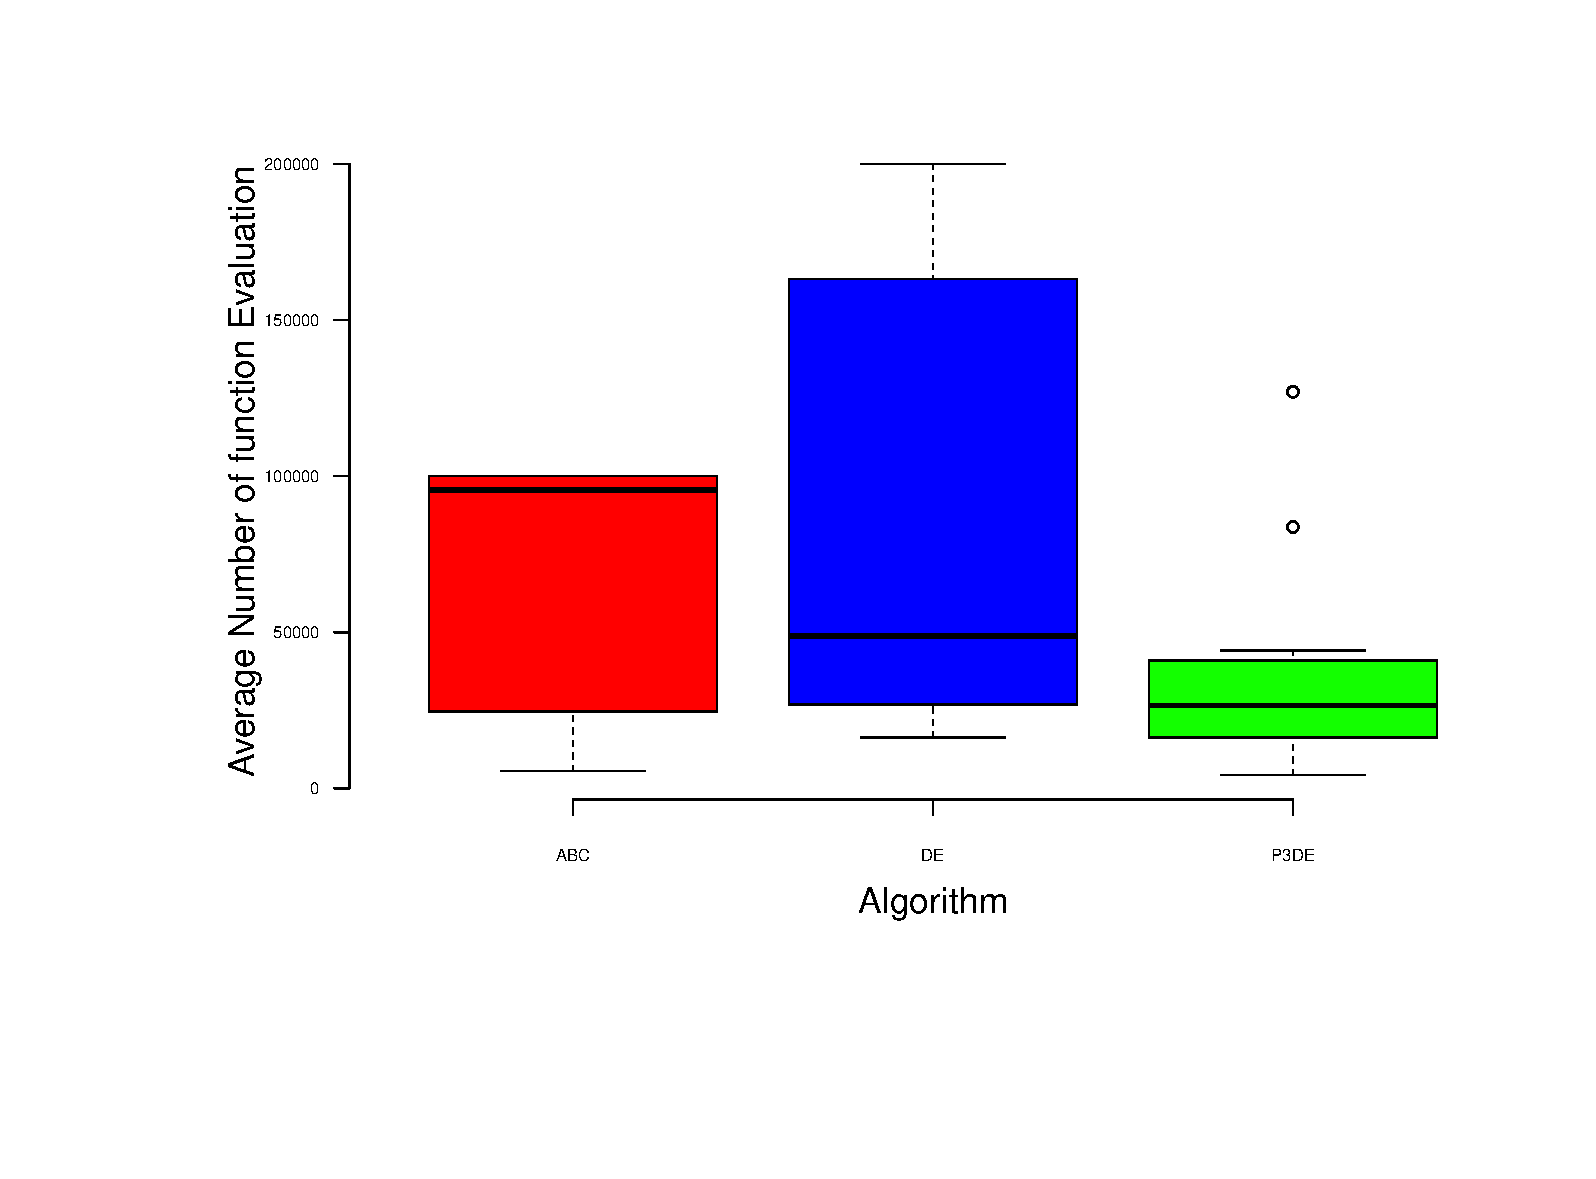
\includegraphics[width=0.9\textwidth]{Boxplot.eps}
    \caption{Boxplots graph for AFE}
     \label{fig:bp_feval}
\end{center}
\end{figure}


Further, a fair comparison in terms of the convergence speed is done through AR analyses on the AFEs of the considered algorithms. The AR is calculated by equation \ref{lsabceq:ar}.

\begin{equation}\label{lsabceq:ar}
    AR=\frac{AFE_{ALGO}}{AFE_{P3DE}},
\end{equation}
where, ALGO$\in$ \{DE and ABC\}.
It is clear from equation \ref{lsabceq:ar} that the AR will be high for the algorithm having fewer AFEs and vice-versa. The calculated AR is presented in Table \ref{lsabctable:ar}. While observing the Table \ref{lsabctable:ar}, the value of AR is more than one for most of the function which shows that the newly developed P3DE is fast convergent algorithm as compared to the other considered algorithms.

\section{Conclusion}\label{sec:con}
A new modification in DE algorithm is suggested in this paper and named as Peregrine Preying Pattern based DE (P3DE) algorithm. The newly anticipated strategy is inspired by a unique pattern followed by peregrine falcon while chasing its prey that is depicted as logarithmic spiral. The exploration capability of the DE algorithm is improved by the logarithmic spiral search process. To assess the anticipated P3DE algorithm, $12$ benchmark functions are selected for experiments. Results proved that P3DE will be a better choice for optimization problems.

\bibliographystyle{plain}
%\fontsize{10}{10}\selectfont
%\addcontentsline{toc}{section}{\textbf{REFERENCES}}
%\renewcommand{\bibname}{REFERENCES}
\bibliography{review}
%\end{spacing}
\end{document}
